\documentclass[12pt]{article}

\usepackage{scicite,times,graphicx,float,hyperref}
\usepackage[skip=0pt]{caption}
\usepackage[utf8]{inputenc}
\usepackage{enumitem}
\usepackage{booktabs}

\topmargin -1.0cm
\oddsidemargin 0.0cm
\textwidth 16cm 
\textheight 23cm
\footskip 1.0cm

\newenvironment{sciabstract}{%
\begin{quote} \bf}
{\end{quote}}

\newcounter{lastnote}
\newenvironment{scilastnote}{%
  \setcounter{lastnote}{\value{enumiv}}%
  \addtocounter{lastnote}{+1}%
  \begin{list}%
  {\arabic{lastnote}.}
  {\setlength{\leftmargin}{.22in}}
  {\setlength{\labelsep}{.5em}}
}
{\end{list}}

\title{A Farm Simulation\\using Swing and Concurrency} 

\author
{Filipe Pires [85122], João Alegria [85048]\\
\\
Software Architecture\\
\normalsize{Department of Electronics, Telecommunications and Informatics}\\
\normalsize{University of Aveiro}\\
} 

\date{\today{}}

%%%%%%%%%%%%%%%%% END OF PREAMBLE %%%%%%%%%%%%%%%%

\begin{document} 

\baselineskip18pt

\maketitle 

\section{Introduction} %%%%%%%%%%%%%%%%%%%%%%%%%%%%%%%%%%%%%%%%%%%%%%%%%%%%%%%%%%%%%%%%%%%%%%%%%%%%%%%%%%%%%%%%%%%%%%%%%%%%%%%%%%%%%%%%%%%%%%%%%%%%%%%%%%%%%%%%%

This report aims to describe the work developed for the first assignment of the course of 'Software Architecture', explaining the overall architecture and 
describing its components and respective communication channels and elaborating on the adopted solutions for concurrency.
We also mention how the work was distributed amongst the authors.

The Java application has the purpose of conducting harvest simulations on an agricultural farm.
Along with the technical aspects of the implementation, we also elaborate on the adopted solutions for concurrency.
Efforts on making the UI highly usable and the code readable and well documented are also stated here.
All code developed is publicly accessible in our GitHub repository:
\url{https://github.com/FilipePires98/AS/}.
\newpage

\section{The Agricultural Farm} \label{farm} %%%%%%%%%%%%%%%%%%%%%%%%%%%%%%%%%%%%%%%%%%%%%%%%%%%%%%%%%%%%%%%%%%%%%%%%%%%%%%%%%%%%%%%%%%%%%%%%%%%%%%%%%%%%%%%%%%%

Agricultural farms have well defined seasons where different activities must be executed to maintain the business productive.
Tasks must be distributed amongst workers and quantities must be calculated and tracked for the correct functioning of the entire farm.
As the whole system grows, its complexity and difficulty in management grows as well, so management tools emerge as valuable assets for farmers.

Amongst the many features of such tools, one offers a particularly interesting view of the farm as it simulates its behavior.
Such simulations allow farm owners to plan harvests and test strategies to understand which offer the greatest productivity and profit.
These simulator tools may be as complex as the farm itself, but allow manipulation of time and other resources without any cost.
So, it is easy to understand that solutions of this nature offer value to the farming audience in general.

With this in mind, it was proposed to us to develop an agricultural farm harvest simulator with very simple features in order to apply the knowledge gained 
during the course.
This simulator isn't meant to serve as a final product for an agricultural business, rather it should show the potential of such solutions.
As it implements concurrency by design, it ensures scalability for a potential product and offers realistic aspects on the virtual farmers' behavior.

But how exactly is the system organized?
There are two main entities: the Control Center (CC) and the Farm Infrastructure (FI). 
The CC is responsible for supervising the harvest, while the FI is the infrastructure for the agricultural harvest.

\subsection{Control Center} %%%%%%%%%%%%%%%%%%%%%%%%%%%%%%%%%%%%%%%%%%%%%%%%%%%%%%%%%%%%%%

The Control Center is where the number of farmers to be used is defined, along with their maximum speed, the amount of existing corn cobs and a special parameter 
called timeout.
Timeout, defined in milliseconds, is a parameter used for regulation of the simulation's execution time and sets the maximum amount of time for each farmer to 
make a movement.

It is in the CC that users send orders for the virtual farmers to execute.
The commands available are:
\vspace{-10pt}
\begin{itemize}[noitemsep]
  \item Prepare - the selected farmers move to a Standing Area, ready for orders.
  \item Start - the actual simulation begins and farmers start moving.
  \item Collect - farmers collect corn cobs from the Granary (where the cobs initially are).
  \item Return - farmers return to the Storehouse with the collected corn cobs.
  \item Stop - farmers stop whatever they are doing and return to the Storehouse.
  \item Exit - simulation ends and the program closes.
\end{itemize}
\vspace{-10pt}

\subsection{Farm Infrastructure} %%%%%%%%%%%%%%%%%%%%%%%%%%%%%%%%%%%%%%%%%%%%%%%%%%%%%%%%%

The Farm Infrastructure is the part of the system that has the virtual components of the farm.
It holds four sections of the farm:
\vspace{-10pt}
\begin{itemize}[noitemsep]
  \item Storehouse - where farmers rest and corn cobs are stored.
  \item Standing Area - where selected farmers wait for further orders.
  \item Path - a representation of the field that farmers must cross.
  \item Granary - where corn cobs are temporarily stored.
\end{itemize}
\vspace{-10pt}
FI also supports virtual farmers, which during their lives transit between the following states:
\vspace{-10pt}
\begin{itemize}[noitemsep]
  \item Initial - resting (blocked) in the Storehouse.
  \item Prepare - ready for orders (blocked) in the Standing Area.
  \item Walk - moving in the Path (one by one, in the same order they entered it) towards the Granary.
  \item Wait to Collect - waiting for orders (blocked) to collect corn cobs in the Granary.
  \item Collect - collecting corn cobs from the Granary.
  \item Return - moving in the Path (one by one, in the same order they entered it) towards the Storehouse, with the collected cobs.
  \item Store - storing the collected corn cobs in the Storehouse.
  \item Exit - farmer kills itself.
\end{itemize}
\vspace{-10pt}
So, as you can see, there is a direct mapping between the commands made available to users and the farmer states.
\newline 

When deployed, the system offers a Graphical User Interface (GUI) for each entity.
CC's UI allows user interaction and FI's UI allows visualization of the simulation in real time.
We added to CC's interface a mirror of FI's to allow the possibility of both entities running in different environments far away from each other, while ensuring 
that the user on CC's side has knowledge of what is happening during the simulation.
This and other interface-related aspects will be mentioned in greater detail further ahead.

\begin{figure}[H]
  \centering
  \begin{minipage}{\textwidth}
    \centering
    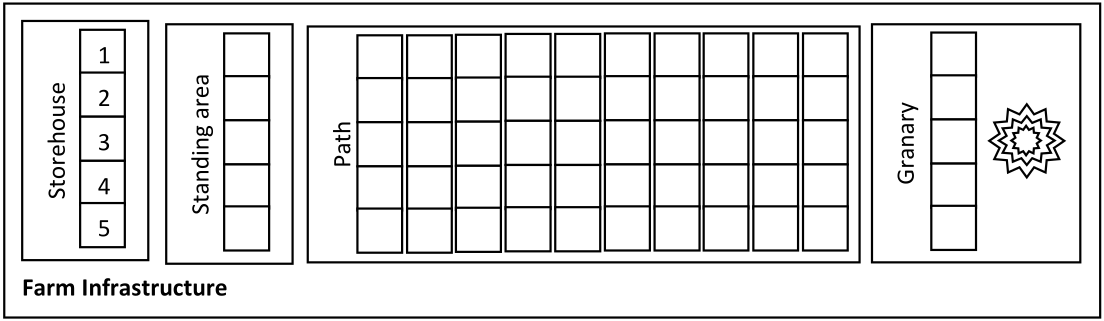
\includegraphics[width=\linewidth]{FarmSimulation_FarmDesign.png}
  \end{minipage}%
  \caption{Visual representation of the farm, taken from \cite{assign}.}
  \label{class_diagram}
\end{figure} 

\newpage
\section{System Architecture} %%%%%%%%%%%%%%%%%%%%%%%%%%%%%%%%%%%%%%%%%%%%%%%%%%%%%%%%%%%%%%%%%%%%%%%%%%%%%%%%%%%%%%%%%%%%%%%%%%%%%%%%%%%%%%%%%%%%%%%%%%%%%%%%%%

In this chapter we focus on the implementation of each component and on the architecture of the entire solution.
Here, we resort to a class diagram (see Figure \ref{class_diagram}) to visually aid interpretation.
We also present screenshots of the GUIs to explain how the interaction works.

Our harvest simulator follows a modular structure implemented in Java.
As we will see, each component has a specific purpose and is responsible for one key aspect of the system's functionality.
The principle of least knowledge is here applied and code dependency is kept low.
This means that there are no unnecessary elements but it is needless to say that without any of the components the system will not work as intended.
The system is designed to be extensible as well, through the use of well defined interfaces that allow the insertion of new elements such as new farm areas or 
even different types of farmers.

All relevant actions during simulations are printed to a unique terminal, with the due source identification, allowing an easy management of what is occurring 
during execution.
To deal with exceptions thrown by user commands, we designed our own exception handling mechanisms.
Also, since the user side is the greatest potential source of errors, the interface is confined to its most limited usage, i.e. users are only allowed to do 
what they can actually do at all times.
Although this may seem to reduce the usability of the solution, it actually helps users by guiding them towards what they can and want to do, without leaving 
margin for errors.

Components belonging to the same logical layer are grouped within a package.
Interfaces, classes and methods are all documented, with the help of Javadoc, and naming conventions are applied throughout the code, focusing on allowing readers 
to understand what methods and variables do by reading their names alone.
Communications between independent components are done through defined protocols. 

\subsection{Components} %%%%%%%%%%%%%%%%%%%%%%%%%%%%%%%%%%%%%%%%%%%%%%%%%%%%%%%%%%%%%%

Let us now go deeper into each component in order to understand how the execution flow is conducted.
Once the Java application is executed, out Main class launches a subprocess dedicated to the FarmInfrastructure and instantiates the ControlCenter, passing full 
control to it.
Every Java application has a single instance of class java.lang.Runtime that allows the application to interface with the environment in which it is running.
By obtaining the environment through \textit{Runtime.getRuntime()} and calling the \textit{Runtime.exec(String command)} method, the Main class is able to launch 
an independent Java process and manage it - allowing the existance of the previously mentioned unique terminal for printing system status during runtime.
The \texttt{command} string is built by retrieving the directory where the code is located: 

\texttt{java -cp <userdir>/build/classes fi.FarmInfrastructure}

\begin{figure}[H]
  \centering
  \begin{minipage}{\textwidth}
    \centering
    \includegraphics[width=\linewidth]{FarmSimulation_ClassDiagram.png}
  \end{minipage}%
  \caption{Class diagram of the Farm Simulation application.}
  \label{class_diagram}
\end{figure} 

Now we have our two entities - the system's core.
ControlCenter and FarmInfrastructure implement the UiAndMainControlsCC interface and UiAndMainControlsFI interface respectively.
Both classes extend from \texttt{javax.swing.JFrame} and contain the code regarding the GUIs and communicate with each other with the use of sockets.
Both have instances of SocketServer and SocketClient and work as servers and clients simultaneously.
The communication establishment is explained in section \ref{communications}.

MonitorMetadata and 4 Monitors (and respective interfaces)

Farmer and FarmerState

Exceptions

........ 



\subsection{User Interface} %%%%%%%%%%%%%%%%%%%%%%%%%%%%%%%%%%%%%%%%%%%%%%%%%%%%%%%%%

........

\newpage
\section{Concurrency Strategy} %%%%%%%%%%%%%%%%%%%%%%%%%%%%%%%%%%%%%%%%%%%%%%%%%%%%%%%%%%%%%%%%%%%%%%%%%%%%%%%%%%%%%%%%%%%%%%%%%%%%%%%%%%%%%%%%%%%%%%%%%%%%%%%%%

..... 

\subsection{Communications} \label{communications} %%%%%%%%%%%%%%%%%%%%%%%%%%%%%%%%%%

........

SocketClient, SocketServer, CCMessageProcessor and CCProxy, ProcessingThread (and MessageProcessor interface)

\subsection{Farmers} %%%%%%%%%%%%%%%%%%%%%%%%%%%%%%%%%%%%%%%%%%%%%%%%%%%%%%%%%%%%%%

........

%%%%%%%%%%%%%%%%%%%%%%% FIGURE %%%%%%%%%%%%%%%%%%%%%%%%%%%

% \begin{figure}[H]
%   \centering
%   \begin{minipage}{\textwidth}
%     \centering
%     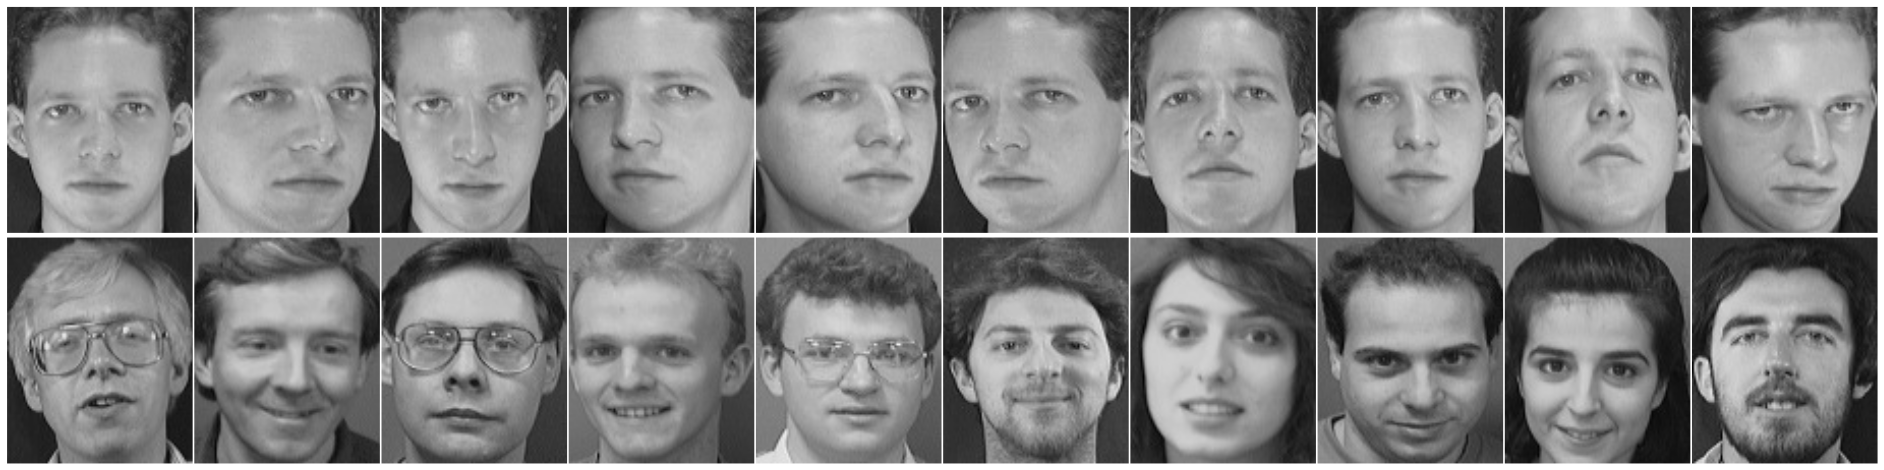
\includegraphics[width=\linewidth]{faces_example.png}
%   \end{minipage}%
%   \caption{Image taken from the assignment description \cite{trab3}. Examples from the ORL face dataset. In the first row, ten face images corresponding to the same subject (s01). In the second row, the first face image of subjects s02 to s11.}
%   \label{fig:1}
% \end{figure}

%%%%%%%%%%%%%%%%%%%%%%%% LIST %%%%%%%%%%%%%%%%%%%%%%%%%%%%%

% \vspace{-10pt}
% \begin{itemize}[noitemsep]
%   \item Append - this operation unites the two images one above the other (duplicating the height of the resulting image).
%   \item Interlace - interpolated horizontal stripes of both images are stacked together (in this operation half of the data of each image is not used).
%   \item Average - for each pixel position, the average of the gray value of both images at that position is calculated and added to the new image in the same position.
% \end{itemize}
% \vspace{-10pt}

%%%%%%%%%%%%%%%%%%%%%%%% TABLE %%%%%%%%%%%%%%%%%%%%%%%%%%%%

% \begin{table}[h!]
%   \centering
%   \begin{tabular}{@{}c|cccccc@{}}
%                      & \textbf{\texttt{zip}} & \textbf{\texttt{gzip}} & \textbf{\texttt{lzma}} & \textbf{\texttt{bzip2}} & \textbf{\texttt{zpaq}} & \textbf{\texttt{ppmd}}\\ \midrule
%   \textbf{Append}    & 0.707     & \textbf{0.725}   & 0.271           & 0.507     & 0.060           & 0.657 \\
%   \textbf{Interlace} & 0.100     & 0.560            & \textbf{0.682}  & 0.578     & 0.021           & 0.025 \\ 
%   \textbf{Average}   & 0.021     & 0.021            & 0.014           & 0.042     & \textbf{0.089}  & 0.025 \\ 
%   \end{tabular}
%   \vspace{5pt}
%   \caption{Accuracy for each compressor using different concatenation operations.}
%   \label{tab:1}
%   \end{table}

%%%%%%%%%%%%%%%%%%%%%%% EQUATION %%%%%%%%%%%%%%%%%%%%%%%%%%%

% \begin{equation} \label{eq:1}
%   NID(x,y) = \frac{max\{K(x|y),K(y|x)\}}{max\{K(x),K(y)\}}
% \end{equation}

%%%%%%%%%%%%%%%%%%%%%%%%% CODE %%%%%%%%%%%%%%%%%%%%%%%%%%%%%

% \begin{verbatim}
%   for each compressor, do:
%     for each subject, do:
%       minNCD = 1
%       for each testImg, do:
%         for each goldStdImg, do:
%           tmp = concat(testImg,goldStdImg)
%           cTmp = compress(tmp)
%           cT = compress(testImg)
%           cGS = compress(goldStdImg)
%           maxS = getMaxSize(cTmp,cT,cGS)
%           minS = getMinSize(cTmp,cT,cGS)
%           NCD = (size(cTmp) - minS) / maxS
%           if NCD < minNCD:
%             minNCD = NCD
% \end{verbatim}

% \vspace{0.2in}
% \begin{minipage}{0.45\textwidth}
%   \begin{verbatim}
%     def stringA():
%       for i in range(5):
%         print("01", end="")
%   \end{verbatim}
% \end{minipage}
% \begin{minipage}{0.45\textwidth}
%   \begin{verbatim}
%     def stringB():
%       for letter in "0010100110":
%         print(letter, end="")
%   \end{verbatim}
% \end{minipage}
% \vspace{0.2in}

%%%%%%%%%%%%%%%%%%%%%%%%%%%%%%%%%%%%%%%%%%%%%%%%%%%%%%%%%%%%

\newpage
\section{Documentation} %%%%%%%%%%%%%%%%%%%%%%%%%%%%%%%%%%%%%%%%%%%%%%%%%%%%%%%%%%%%%%%%%%%%%%%%%%%%%%%%%%%%%%%%%%%%%%%%%%%%%%%%%%%%%%%%%%%%%%%%%%%%%%%%%%%%%%%%

.....

\newpage
\section{Discussion} %%%%%%%%%%%%%%%%%%%%%%%%%%%%%%%%%%%%%%%%%%%%%%%%%%%%%%%%%%%%%%%%%%%%%%%%%%%%%%%%%%%%%%%%%%%%%%%%%%%%%%%%%%%%%%%%%%%%%%%%%%%%%%%%%%%%%%%%%%%

.....

Regarding the work distribution amongst developers, a close-contact strategy was defined where each worked on a piece of software according to a predefined plan. 
The project structure and architecture was decided in conjunction, as well as the key concurrency solutions chosen.
Both servers were also implemented collectively.

Nevertheless, some relatively independent task distribution was defined: João implemented the Granary and Path monitors, while Filipe did the Storehouse and 
Standing monitors; João established socket communications and respective message processors, while Filipe designed the user interface and respective interaction
with the remaining components.
Bug and error solving was made along the development phase by both developers any time it was required.

Once the final version of the application was completed, this report and the code documentation became our primary concern, with both contributing equally.


\newpage
\section{Conclusions} %%%%%%%%%%%%%%%%%%%%%%%%%%%%%%%%%%%%%%%%%%%%%%%%%%%%%%%%%%%%%%%%%%%%%%%%%%%%%%%%%%%%%%%%%%%%%%%%%%%%%%%%%%%%%%%%%%%%%%%%%%%%%%%%%%%%%%%%%%

After completing the assignment, we drew a few conclusions regarding the topics here explored and our endeavor to deliver work of quality.

.....

\begin{thebibliography}{9} %%%%%%%%%%%%%%%%%%%%%%%%%%%%%%%%%%%%%%%%%%%%%%%%%%%%%%%%%%%%%%%%%%%%%%%%%%%%%%%%%%%%%%%%%%%%%%%%%%%%%%%%%%%%%%%%%%%%%%%%%%%%%%%%%%%%%
  \bibliographystyle{Science}

  \bibitem{assign}
    Óscar Pereira,
    \textit{SA: Practical Assignment no.1},
    University of Aveiro,
    2019/20.
  
  % \bibitem{imgmagick}
  %   ImageMagick Studio LLC,
  %   \textit{ImageMagick},
  %   \url{https://imagemagick.org/index.php},
  %   accessed in December 2019.

  % \bibitem{lzmaExplanation}
  %   Borbely, R.,
  %   On normalized compression distance and large malware: Towards a useful definition of normalized compression distance for the classification of large files,
  %   Journal of Computer Virology and Hacking Techniques,
  %   2015,
  %   10.1007/s11416-015-0260-0
  %   \url{https://www.researchgate.net/publication/290319316_On_normalized_compression_distance_and_large_malware_Towards_a_useful_definition_of_normalized_compression_distance_for_the_classification_of_large_files},
  %   accessed in December 2019.
  
\end{thebibliography}

\clearpage

\end{document}




















